\section{Religion}
On Athas, true gods don't exist, but this fact has never stopped its inhabitants from having faith and religions. Most devote themselves to a specific element, others to nature as a whole, and a few others pray to their sorcerer-kings.

A pterran psychic warrior who prays to Earth Mother and a thri-kreen druid often share the same world views, even though their faiths are not exactly the same. An elf rogue devotee of the element of Air and an aarakocra Air cleric are members of the same religion: they may differ in many respects, certainly in alignment and ethics, but they do not see religion as one of the lines dividing them.

\textbf{Race and Religion:} The religions of Athas are not, in general, racially based. Only pterrans, ssurrans, and a few other races have religions that are rarely practiced by members of other races. The other races share a number of religions that welcome clerics and adherents of all races and origins.

\subsection{The Elements}
\begin{figure*}[b!]
\centering
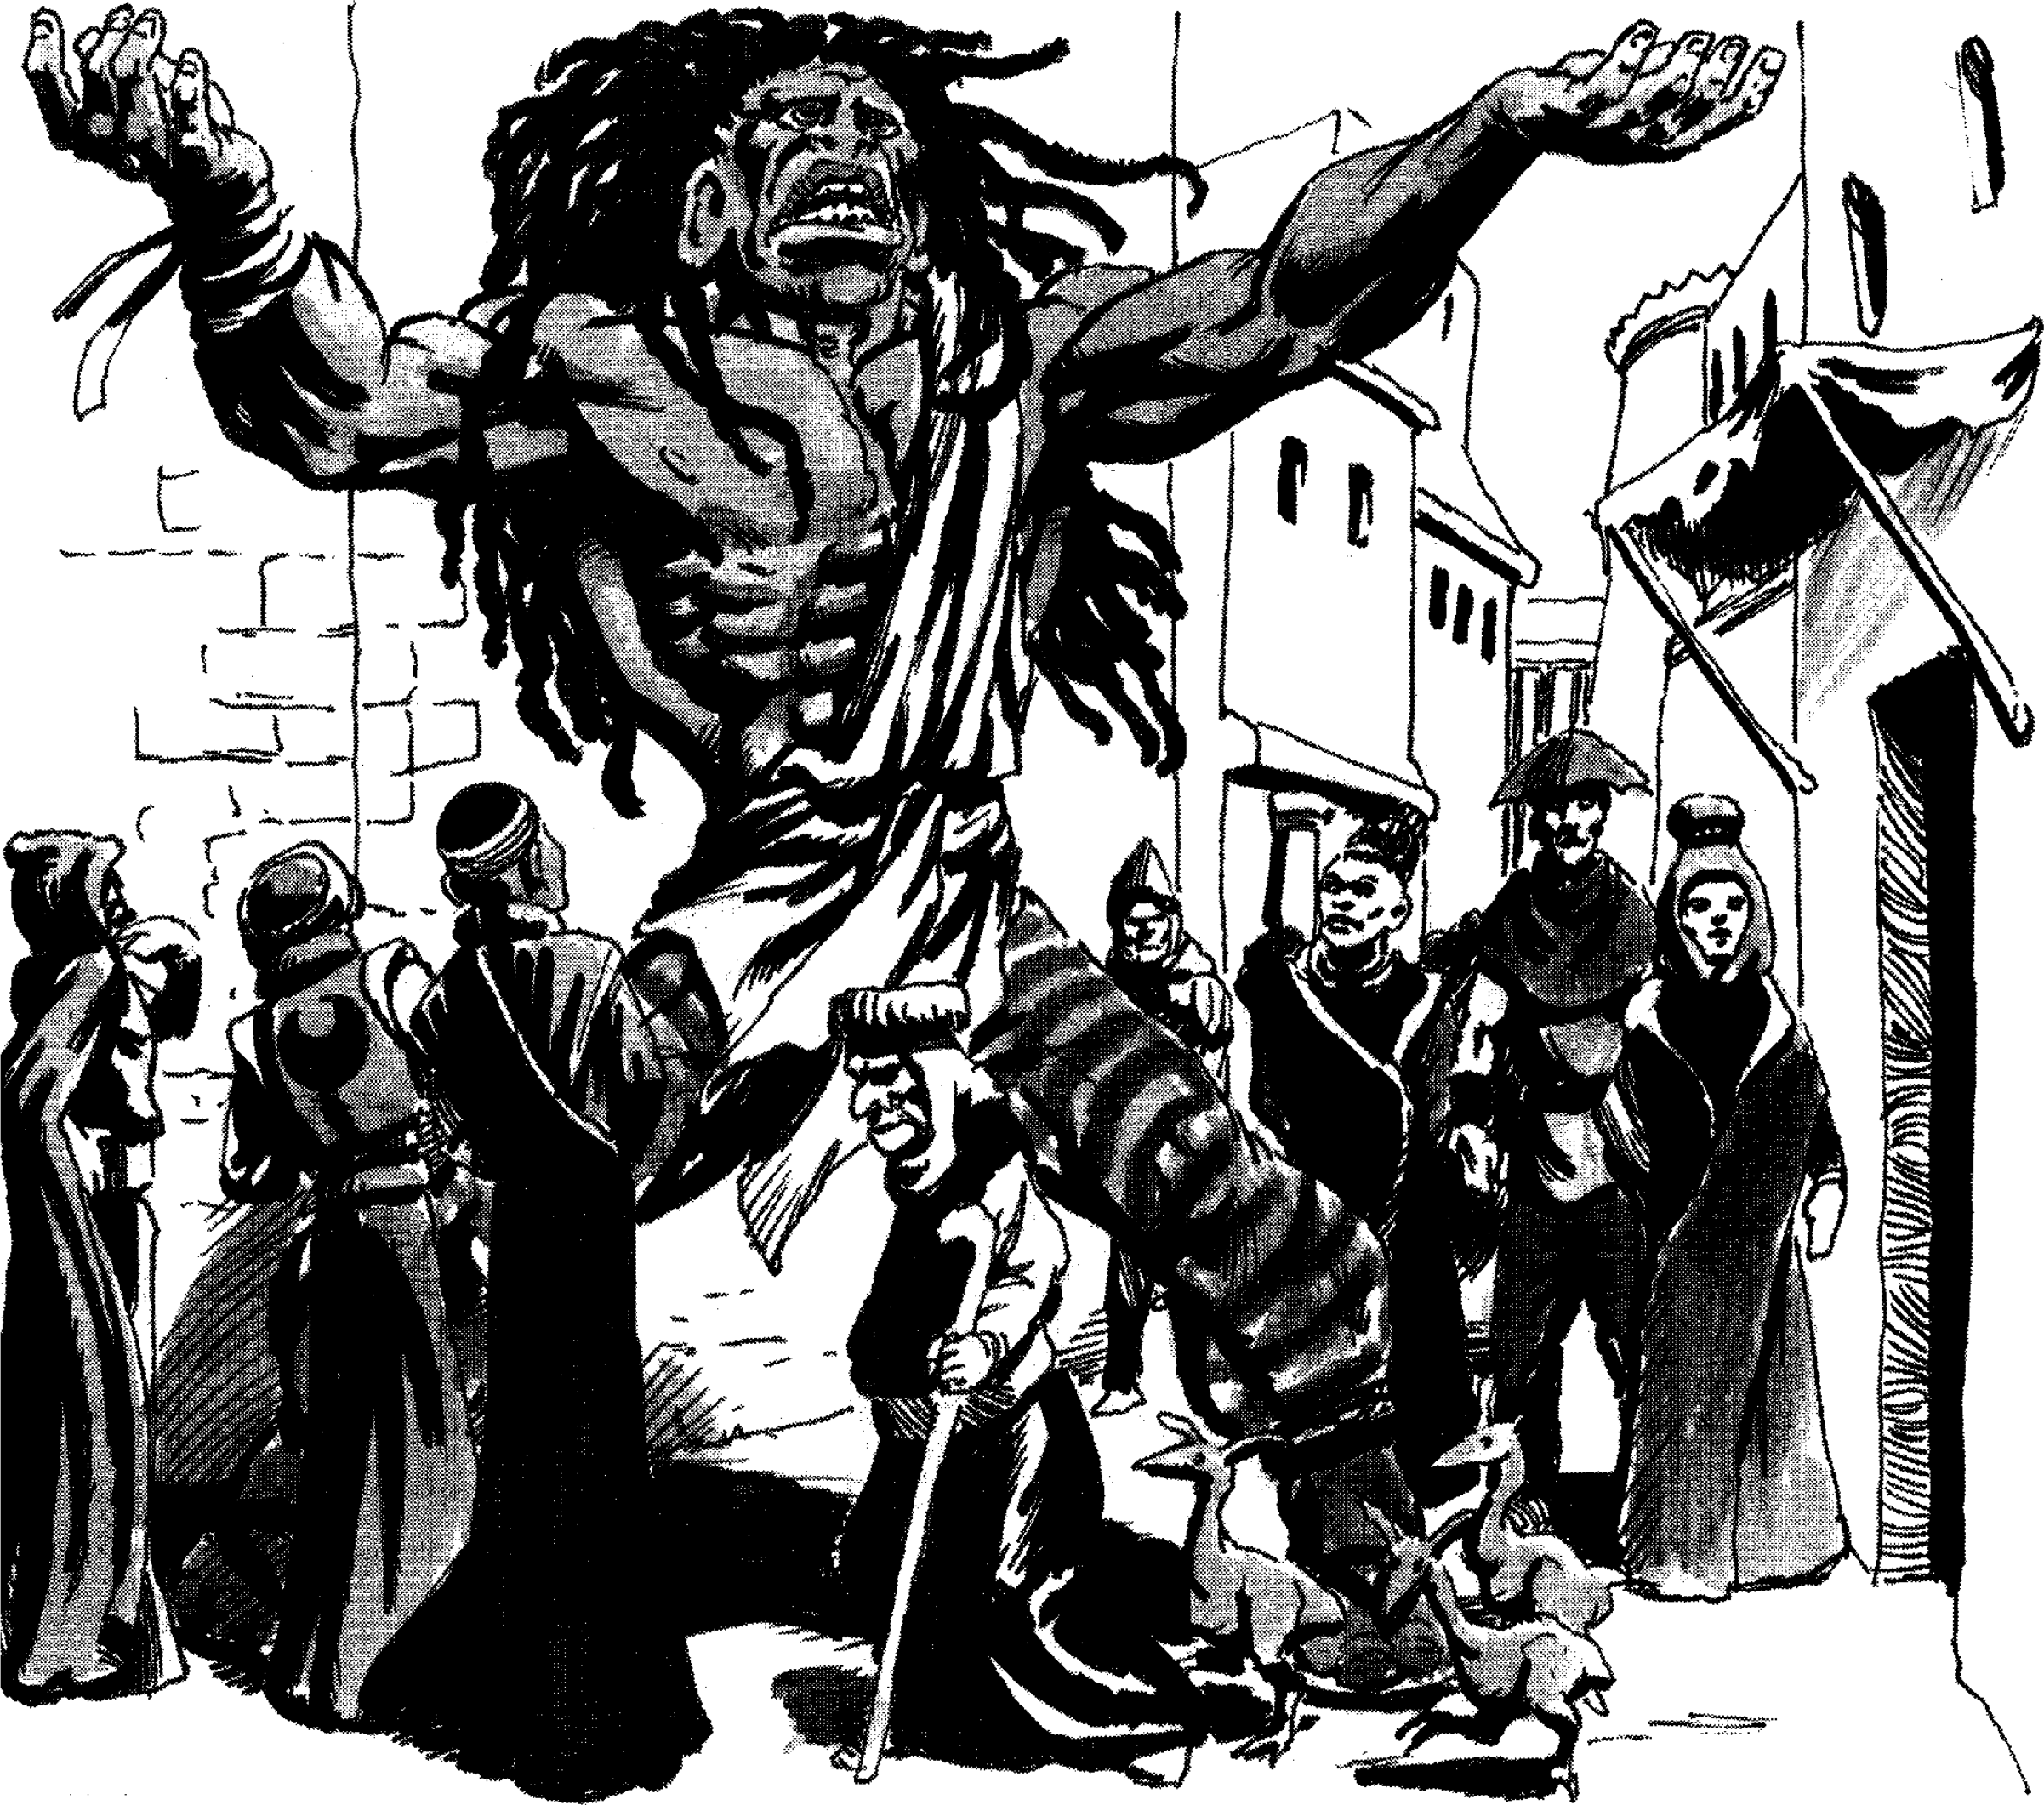
\includegraphics[height=0.4\paperheight]{images/halfgiant-2.png}
\par\textit{\small\textcopyright Wizards of the Coast, 2020.}
\end{figure*}

Elemental magic is a common source on Athas. Due tothe connection between Athas and the elemental planes,the powerful beings that dwell there will aid individualson Athas if they pledge to support their patron's element. Elemental priests exist in the city-states, in villages in thewastes, and along barren tracks of desert and scrub brush.Wherever people are found, they can be foundworshiping the elements.

\subsubsection{Air}
Clerics devoted to Air are found wherever the wind affects people's lives. Clerics of air help their communities by using wind turbines to grind grain, by taking the roles of seers by listening to the winds, and by bringing freedom to elf tribes by never staying in one place and going where the wind blows. Worshipers of Air are like the wind, their minds are constantly wandering. They rarely seem focused on a current problem or situation. The most important principle to clerics of Air is freedom. They loathe restrictions on their movement, beliefs, practices, even clothing and food. Air clerics rebel against any attempts to impose such limitations on themselves or others.

\subsubsection{Earth}
Those who worship earth tend to care about the soil and the land. Of all the elemental clerics, they seem to take the longest view, knowing that time spent now investing n the future can take years to come to fruition. They hate defilers more than any other Elemental clerics. They find themselves concerned with farming, crop rotation, and building projects. Their view of time makes them excellent planners. They also deal often with the dead, as they see death as a tragic but necessary stage in nature's endless chain of life. People will trust that those buried by the worshipers of Earth won't rise from the grave.

\subsubsection{Fire}
Of all the elemental clerics, fire is the most temperamental. While some are pyromaniacs, burning all they can and looking for destruction in all things, most take a more pragmatic view of the world. They know that the fiery passion they feel needs something to ignite. They often help with the planting of trees and the clearing of scrub brush. In the north, they enjoy the Burning Plains south of the Last Sea. When it comes to farming, they know that the ash left behind after a brush fire makes the crops grow faster and heartier. Finally, they are sometimes seen at funerals for those who don't choose to trust their dead to the earthen embrace. In cities, the fire worshipers are often in charge of the city crematory, as they can dispose of bodies without the need for space.

\subsubsection{Water}
Water is the giver of life, but the elemental lords of water now perform this task grudgingly. The Elemental Plane of Water has lost more than any of the others to the ravages of defiling. The Lords of Water demand that their clerics preserve and protect the water that remains. Despite this, it remains the duty of water clerics to give a water to any in need. As such, those who worship Water are seen as some of the most beneficial to communities. Where water clerics go, so too do they bring the ability to summon forth the element that they worship. Because of the shortage of water on Athas, water clerics are seen as wonder workers and miracle men. They help find water in the wastes for tribes on the go, help dig wells in cities and villages to ensure the community will survive, and help to purify water that an elf tribe frequents to ensure that it will be there on their next visit. Almost all people on Athas hold water worshipers in high esteem, as they can provide something that is needed in almost every community.

\subsection{The Paraelements}
Paraelemental worshipers are a varied lot. Because their patrons are concerned more with power than responsibility, the destructive nature of these Lords is feared by many. However, this is not always the case, as sometimes worshipers of these elements will work to protect a village from these elements instead of causing chaos.

\subsubsection{Magma}
Volcanic activity is relatively rare on Athas. That said, the land around Urik, and the Road of Fire is home to many who venerate Magma as a source of power. Magma clerics are elite warriors within the Urikite army, traders within the Road of Fire, and miners of obsidian for merchant houses and protectors of the farming villages around volcanic lands whose soil is rich and fertile.

\subsubsection{Rain}
Rain is the weakest element on Athas, even after the development of the Cerulean Storm. Rain worship is common in halfling villages in the Ringing Mountains, as it helps the jungle to grow and provide nourishment. Outside of these forest environments, rain clerics are found rarely in the wastes, bringing what little rain they can to starved villages.

\subsubsection{Silt}
Silt worshipers are found all along the Silt Sea. They protect villages by keeping the silt at bay, and they work for merchant houses by finding safe passage within the deep silt, and guiding travel and trade. They are also found in the fleets of both Balic and Eldaarich, helping the court navies hunt pirates and giants, using the silt to their advantage. Of course, these pirates and giants have silt priests of their own, and will often raise storms and use the silt against those they wish to attack.

\subsubsection{Sun}
Sun worshipers are seen across the Tablelands. They are quick to anger and are not afraid to scorch those they think have wronged them. Their pack with the Paraelemental Lords requires them to eliminate any obstructions that would defy the sun's rays. Any building, tree, or hill that provides shade is considered an affront to the Sun's harsh embrace. The Paraelemental Lords of Sun would like nothing better than a flat barren landscape in which no creature could find any shade. Elf tribes that venerate the Sun have been known to stake out victims so that they dry out and wither under the blistering rays. A few sun clerics are seen as beneficial to their village or tribe, and know that the sun is the source of all life on Athas.

\subsection{Nature}
Druids tend to be the ones who worship nature, owing their power to the land that they work with. Druids safeguard nature from defilers, seeking to destroy them and maintain the balance in their guarded lands. Druids are as varied in temperament as any other group, with some being violently opposed to any trespasser; while others will welcome those they see as potential allies. Others who work with druids, in various villages in the wastes, can work towards a balance of things and work in harmony with the land they inhabit. Those who venerate nature do so because they see that working with the land is better than stealing from it, and that the Spirits of the Land will protect those who care for them.

\subsection{The Sorcerer-Kings}
The sorcerer-kings are venerated differently, depending on the city state. Some are worshiped as gods, while others are content to have their followers honor them in other ways. Regardless of whether or not they are worshiped as gods, sorcerer-kings are not divine, though they do grant divine spells to their templars from their connection to the elemental planes.

\begin{figure}[t!]
\centering
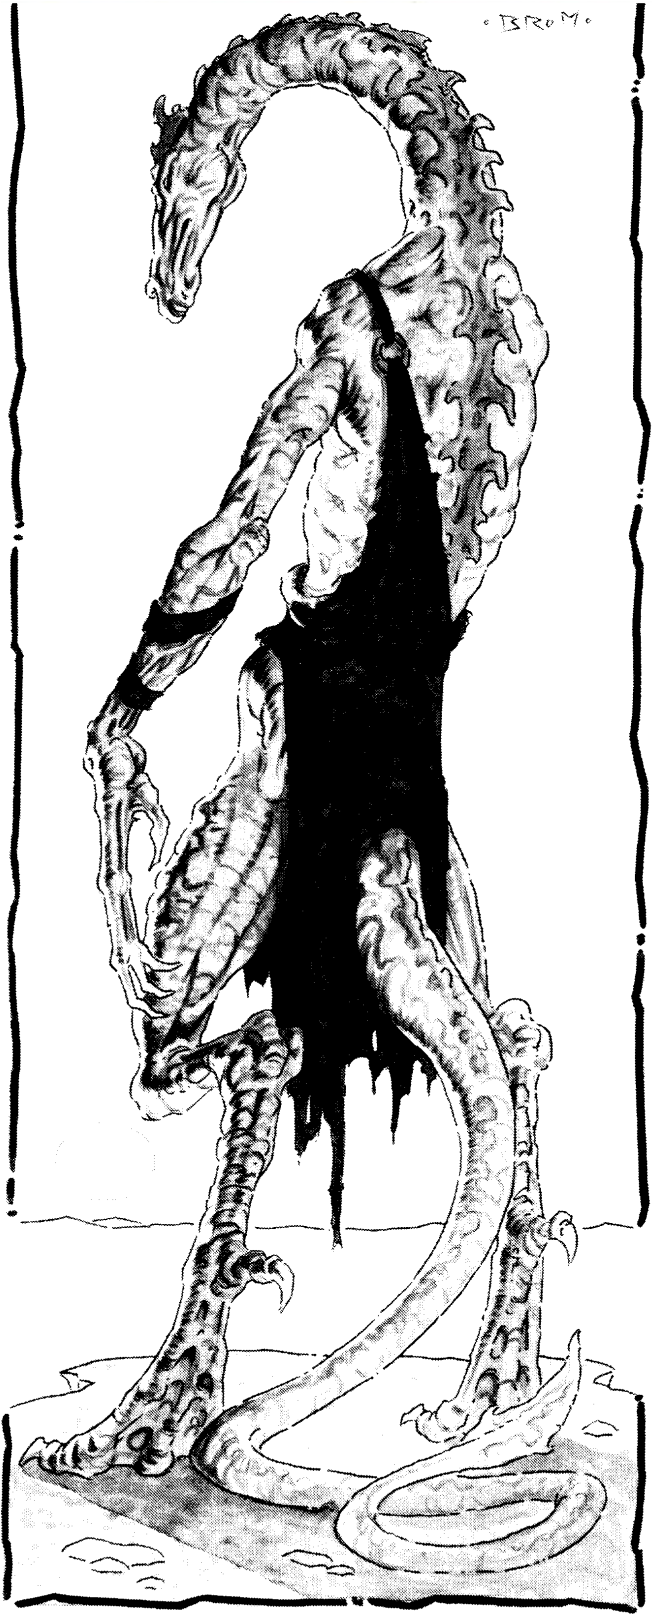
\includegraphics[width=\columnwidth]{images/dragon-2.png}
\par\textit{\small\textcopyright Wizards of the Coast, 2020.}
\end{figure}

\subsubsection{Abalach-Re}
Before her death in FY 10, Abalach-Re called herself the Great Vizier. She claimed to be the representative of Badna, a greater power who bestowed powers upon her. Abalach-Re claimed that Badna would strike her dead if she did not execute her position well. As the head of this religion in the worship of this higher being, she was able to shift the anger of the most volatile city-state away from her and onto Badna. Since her death, Raam has been in chaos, with various religions taking her place. Few of her templars have bothered to continue the worship of Badna, as consolidating power is more pressing at the moment.

\subsubsection{Andropinis}
Before the death of the Dragon, Andropinis ruled Balic as an elected dictator. He held his post for over seven hundred years. His rule was absolute and fierce, which was helpful in his almost constant battles against giants and silt pirates. Anyone who spoke out against his rule was executed while Andropinis informed everyone within earshot that he was elected for a life term. Unfortunately for the citizens of Balic, that proved to be a very long time. Since his imprisonment within the Black, his templars have been scattered to the winds and driven underground. They have recently begun to reconnect with their master, and now draw their power from the plane that he is a prisoner of. There are rumors that they work to find a way for him to escape.

\subsubsection{Borys}
Before the events that led to the creation of the Cerulean Storm and the destruction of Ur Draxa, common Draxans almost worshiped the Dragon, referring to him in the same way a religious fanatic might to the leader of his sect. The Dragon could do no wrong; he was a living example of strength, wisdom, and power to be emulated. Despite the adulation Borys enjoyed, he did not seek deification. Thousands of years ago he could have proclaimed himself a god, but apparently the absolute loyalty of his citizens was sufficient for his purposes until his recent death.

\subsubsection{Daskinor}
Daskinor is not seen as a god by his people. In fact, he is not really seen at all, though his influence is definitely felt. His templars refer to him as ``The Old Spider.'' He rarely leaves his chambers, staying in a state of comatose withdrawal, and awakens only to be in fear of some new threat to his life, which he then mobilizes his city-state against, even if that threat is the city-state itself. Well past the point of madness, Daskinor's rule is one of terror. It is an insane asylum run by the craziest inmates of all, a prison rather than a city.

\subsubsection{Dregoth}
The people of Giustenal were convinced of Dregoth's divine nature even before he rose from the dead as a kaisharga. Returning to walk among them after falling to the sorcerer-kings only served to strengthen their devotion. Later, when he transformed them into the dray, his followers became ``the chosen people''. To this day, their belief in Dregoth has only increased---even among the first generation dray of Kragmorta.

All dray know the prophecy of the Coruscation, the Day of Light. In the future, Dregoth the Godking will lead the dray to the land above. There, they will swarm over a place of evil called Raam, killing all of its inhabitants as sacrifices to Dregoth. On that day, when the blood of thousands of unbelievers runs in rivers at the feet of Dregoth, the crimson sun will burst with bright light and the Day of Light will begin.

\subsubsection{Hamanu}
Hamanu portrays himself as a warrior god. He has never lost a battle when he was personally leading his troops. Within the city of Urik, the whim of the Lion is both a curse and a blessing, depending on how it is bestowed. Hamanu is seen as a fiercely protective and strict lord, whose demands and laws are to be followed. Since the fall of the Dragon, Hamanu has closed his city and claimed that he will protect his citizens from the chaos that has erupted across the Tablelands. So far, his godhood is unquestioned and unchallenged, as he has been able to maintain order and stability in a time of disorder and chaos.

\subsubsection{Kalak}
Before his death at the hands of the heroes of Tyr, King Kalak ruled the city state of Tyr with an iron fist. He never declared himself a god, but rather took the title, the Tyrant of Tyr. Pragmatic and utterly ruthless, Kalak was also the most straightforward of the sorcerer-kings. He placed his own survival above that of his citizens, and it is because of this that the Heroes of Tyr rose up against him. Since his death, he has not been venerated or honored, though rumors persist that a court necromancer has stolen his body and seeks to bring the Tyrant back.

\subsubsection{Lalali-Puy}
The sorcerer-queen of Gulg is called the Oba by her subjects. The Oba is an absolute monarch whose name means ``forest goddess'' in the language of her people. This is not a title she assumed herself, but one that her subjects placed upon her. Lalali-Puy can command anything she wishes and know that she will be instantly obeyed by her people. In their eyes, she is a goddess: they attribute her long life to immortality, and they believe that only a being of supreme power could have the abilities that she displays.

\subsubsection{Nibenay}
Nibenay is a bizarre and enigmatic figure. Called the Shadow King by his subjects, the ruler who gave his city his name stays out of the public eye for extended periods of time. Rumors constantly persisted that he died before the events surrounding the death of the Dragon. All his templars are women, and also his wives. While he does not claim to be a god, his subjects venerate and honor him as a wise, if distant ruler.

Since the death of the Dragon he has taken a more active role in the city, working on improving the army and planting agafari trees to replace those he cuts down. Citizens who may not have seen him more than once in a lifetime now see the Shadow King in his more public displays and interactions. Veneration of the ancients and ancestors is common in Nibenay, and no one is more interested in learning about the past than the Shadow King.

\subsubsection{Oronis}
A marked departure from any of the other sorcerer-kings, Oronis does not seek adoration or veneration. Oronis does not even consider himself a king, instead taking a position of advisor to the council that rules Kurn. This, however, makes the people who benefit from his counsel honor and adore him even more.

Oronis works hard to help his people, and is seen helping and risking much for his people. His templars know that he wants to change things, and also know that knowledge is power. He personally teaches at the psionics academy and considers the School of Spies to be an important part of the city.

His people know how life is outside of Kurn, and are learning about the terrible life lead by the Drylanders and Dimlanders. Refugees from Eldaarich come to Kurn to be volunteers as slaves to escape their past. Oronis accepts those he can, and is seen as wise and benevolent by his people.

\subsubsection{Tectuktitlay}
The sorcerer-king of Draj called himself The Mighty and Omnipotent Tectuktitlay, Father of Life and Master of the Two Moons. Claiming to be a god, he made himself the center of Draj religious ceremony and life. Battle and War were important aspects of this religion, and ritual blood sacrifice was central to the rites of their beliefs. Tectuktitlay's templars, called moon priests, claimed that he raised the city from the mudflat, and that he had ruled since time began.

Since his death, his son Atzetuk has taken the throne. The moon priests continue the rites and rituals in the same manner, connecting them to Ral and Guthay, and to the continued survival of the city. The House of the Mind, Draj's psionic academy has also been influential in maintaining order in the city, though rumors exist of tension between the two groups that advise the New King.

\subsection{Other Religions}
There are other religions that exist besides those of elemental worship or veneration of the sorcerer-kings. Some are specific to a particular race, while others are a throwback to an earlier time.

\subsubsection{Coraanu Star Racer}
Significant elven individuals from past generations are remembered and glorified in song and dance. This is one of the few examples of elven behavior not based on the current moment. In the legends and histories of past heroes, elves find inspiration for the now. Some of these ancient heroes are common to all elves.

Perhaps the greatest of these heroes is Coraanu Star Racer, who supposedly led the elves to Athas and established their most basic traditions. He taught the elves to run, to fight, to use the sword and bow, to steal, to sing, and even to dance. All tribes acknowledge his contributions, and most revere him as the greatest elf ever to run beneath the crimson sun.

\subsubsection{The Cerulean Storm}
A new worship has developed after the events in FY 10, the worship of the forces of the storm. The element of Rain has recently established a small temple in Draj. The recent turbulent events and subsequent Tyr-storms have shaken the population, and many have turned to new forces to find solace or meaning in their lives. The destructive nature of the Tyr-storms have awed many Athasians, but specially Draji, and Rain priests have made sure to use this into their advantage.

\subsubsection{The Great One}
The legend of the Great One, as held in kreen racial memory, is sketchy at best. The racial memory simply tells the thri-kreen that the Great One is to be revered; after the memory has been triggered, the thri-kreen reflexively feels awe and fascination when in the presence of the image, or of an actual avangion. The thri-kreen feel compelled to drop their heads close to the ground, and seek to touch their antennae to the image, or to the edge of an avangion's light aura. The Great One gives thri-kreen a sense of peace and calmness, and removes all aggressive tendencies while they stay in the Great One's presence. Thri-kreen consider images of the Great One-in either thri-kreen or avangion form to be sacred, and worthy of respect, though the word ``holy'' does not quite apply. Those thri-kreen who see the Chak'sa ``remember'' that it is sacred and very old, but have no knowledge of who carved it, or why.

Out in the Hinterlands, ruins exist where undead will tell tales of other, non-kreen Great Ones. Ruins of cities ravaged by time and war have signs of these Great Ones, though little is known of them, if these tales are true at all.

\subsubsection{The Earth Mother}
All pterrans revere the Earth Mother, the name they have given to Athas. They believe that they are the Earth Mother's first, best children, and that the Great Earthquake that happened in FY 10 and the subsequent aftershocks are a call to the Earth Mother's children to get more involved in the affairs of the planet. To this end, explorers have been sent to the east to make contact with other civilizations.

\subsubsection{Astrology}
Many people throughout the Tablelands study and practice astrology. The Merchant's Calendar uses the stars and the lunar cycle to not only designate months, but also for divination and veneration. Some druids worship the night sky, and Air clerics will also pay homage to and participate in astrology. In almost every major city state, and most client villages, a fortune teller will tell you what the stars will guide you to, and what Ral and Guthay will bring the next day.

\subsubsection{The Old Gods}
There are those who talk of the Old Gods, mythical beings that were worshiped in the past and then disappeared. No one knows what happened to these entities, and clerics and templars today claim them to be false. In ancient ruins one can find evidence of their worship, either through murals or writings, or even some undead lurking in the shadows. Some say that they were powerful beings, like the sorcerer-kings, able to grant spells to their followers. Others say that they were merely aspects of the Elements, with a god of the Forge being nothing more than a patron of fire. The truth might be out there, hiding in the next ruin or over the next dune.